\subsection{Pruning Heuristics}
\label{subsec:heuristic}

In the face of uncertainty between a possible
protocol violation and sniffer imperfection, augmented transitions provide the
ability to blame the latter. The exhaustive nature of
Algorithm~\ref{alg:search} means that it always tries to blame sniffer
imperfection whenever possible, making it reluctant to report true
violations.

Inspired by the \textit{directed model checking}~\cite{edelkamp2008survey}
technique which is to mitigate the state explosion problem, we propose to enforce extra
constraints on the mutation trace to restrict the search to only mutation traces
with high likelihood. The modified \texttt{EXTEND} function checks certain
likelihood constraints on the prefix of the mutation trace before continuing
(line~\ref{alg:search:stop}), and stops the current search branch immediately if
the prefix seems \textit{unlikely}.  Because of the recursive nature of the
algorithm, other branches which may have a higher likelihood can then be
explored.

The strictness of the likelihood constraint represents a trade-off between
precision and recall of validation. The more strict the constraints are, the
more false positive violations will potentially be reported, hence the lower the
precision yet higher recall. On the contrary, the more tractable the
constraints are, the more tolerant the search is to sniffer imperfection, hence
the more likely that it will report true violations, thus higher precision but
lower recall.

The exact forms of the constraints may depend on many factors, such as the
nature of the protocol, properties of the sniffer, or domain knowledge.  Next,
we propose two \textit{protocol oblivious} heuristics based on the sniffer loss
probabilities and general protocol operations. Both heuristic contains
parameters that can be fine tuned in practice.

\subsubsection{$\mathit{NumMissing}(d, l, k)$}

This heuristic states that the number of missing packets from device $d$ in any
sub mutation traces of length $l$ shall not exceed $k$ ($k \le l$).  The sliding
window of size $l$ serves two purposes. First, $l$ should be large enough for
the calculated packet loss ratio to be statistically meaningful.  Second, it
ensures that the packet losses are evenly distributed among the entire packet
trace.

The intuition behind this heuristic is that the sniffer's empirical packet loss
probability can usually be measured before validation. Therefore, the likelihood
that the sniffer misses more packets than prior measured loss ratio is quite
low. The value of $l$ and $k$ can then be configured such that $k/l$ is marginally
larger than the measured ratio.

\begin{comment}
In addition, we note that for a fixed $l$, a single threshold $k$ may not work
for traces collected by sniffers with different packet loss probabilities.
Intuitively, sniffers with high loss probabilities require a larger threshold.
Therefore, we perform a \textit{stratified} search with an increasing sequence
of thresholds $\{k_1, k_2,\ldots, k_n\}$ ($k_i < k_{i+1}$ for $1 \le i < n$).
At round $i$, the search is restricted by constraint $NumMissing(d, l, k_i)$.
If a mutation trace is found, the search is completed.  Otherwise, we increase
the round number and repeat the search process.  In this way, this heuristic can
automatically adapt to the underlying sniffer packet loss probabilities. And a
violation is declared when no mutation trace can be found with $NumMissing(d, l,
k_n)$.
\end{comment}

\subsubsection{$\mathit{GoBack}(k)$}

This heuristic states that the search should only
backtrack at most $k$ steps when the search gets stuck using only $E$.
The motivation is that many protocols operate as a sequence of independent
transactions, and the uncertainty of previous transactions often do not affect
the next transaction.
For instance, in 802.11 packet transmission protocol, each packet exchange,
include the original, retransmission and acknowledgment packets, constitute a
transaction.
And the retransmission status of previous packets has no effect on the packets
with subsequent sequence numbers, hence need not be explored when resolving the
uncertainty of the packets with new sequence numbers.  Note that we do not
require the protocol to specify an exact transaction boundary, but only need $k$
to be sufficiently large to cover a transaction. 

\begin{comment}
\subsection{Confidence of Correctness}

A run of $S^+$ on sniffer packet trace $Tr$ may yield two conclusions about the
DUT implementation: either ``definitely wrong'' when $S^+$ rejects $Tr$, or
``possibly correct'' when $S^+$ accepts $Tr$. We now quantify the
\textit{confidence} of the implementation correctness in the later case.

Note that the augmented transitions in $S^+$ implicitly embed the assumptions
about packet losses. In particular, Type-1 transitions assume the sniffer
missed certain packets, while Type-2 transitions assume the sniffer
overheard packets that were missed by the DUT. Intuitively, the portion of such
assumptions (hence packet loss \textit{ratios}) in an accepting transition
sequence should match with the true packet loss \textit{probabilities}.
Otherwise, the correctness confidence, despite $S^+$ accepts $Tr$, is low.

Suppose $Tr$ is the sniffer trace and $Tr'$ is its mutation that satisfies $S$.
We can calculate the three packet loss ratios in our model shown in
Figure~\ref{fig:prob}.

\begin{align}
  &Pr_{ds} = \frac{\parallel \{(t,p) \in Tr'\setminus Tr \land p.src = DUT\}\parallel}
  {\parallel \{(t,p) \in Tr' \cup Tr \land p.src = DUT\}\parallel}\\
  &Pr_{es} = \frac{\parallel \{(t,p) \in Tr'\setminus Tr \land p.src = EP\}\parallel}
  {\parallel \{(t,p) \in Tr' \cup Tr \land p.src = EP\}\parallel}
\end{align}where $Tr'\setminus Tr$ is the set of inferred packets that were missed by the
sniffer (Type-1 transitions in $S^+$).

Note that we can not directly calculate the packet loss ratio from Endpoint to
DUT, since there might be packets that were missed by both the sniffer and the
DUT. We can, however, approximate $Pr_{ed}$ using conditional packet loss
probability.

\begin{align}
  \nonumber
  &(1-Pr_{es})\times Pr_{ed} =\\
  &\frac{\parallel \{(t,p) \in Tr\setminus Tr' \land p.src = EP \land p.dest = DUT\}\parallel}
  {\parallel \{(t,p) \in Tr \cup Tr' \land p.src = EP \land p.dest = DUT\}\parallel}
\end{align}The LHS is the probability that a packet sent from the Endpoint to the DUT was
missed by the DUT yet captured by the sniffer. And the RHS is the ratio of
such packets in the mutation trace.


Consider the 802.11 data transmission protocol and the example trace snippet
shown in Figure~\ref{fig:loss}, the packet loss ratios are:
\begin{align*}
  Pr_{ds} &= \frac{\parallel\{\it{DATA}'_0\}\parallel}{\parallel\{\it{DATA}_0, \it{DATA}'_0\}\parallel} = 0.5\\
  Pr_{es} &= \frac{\parallel\emptyset\parallel}{\parallel\{Ack, Ack\}\parallel} = 0\\
  Pr_{ed} &= \frac{\parallel\{Ack\}\parallel}{\parallel\{Ack, Ack\}\parallel\times (1-Pr_{es})} = 0.5
\end{align*}

\begin{figure}[t!]
  \centering
  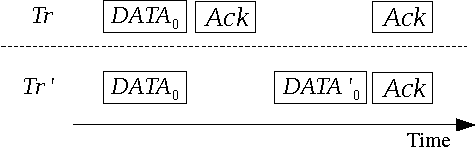
\includegraphics[width=0.4\textwidth]{loss.pdf}
  \caption{\textbf{Example Sniffer Trace and Its Mutation Trace.}}
  \label{fig:loss}
\end{figure}

Suppose we have the true packet loss probabilities $\overline{Pr_{ds}},
\overline{Pr_{es}}$ and $\overline{Pr_{ed}}$, the \textit{confidence} of this
mutation trace $Tr'$ can be defined as:

\begin{align}
  Confidence(Tr') = \prod_{i\in\{ds, es, ed\}}(1-|Pr_i-\overline{Pr_i}|)
\end{align}

By this definition, the trace confidence maximizes when all packet loss
ratios calculated from $Tr'$ matches the true packet
loss probabilities.

Suppose we have $M$ mutation traces that satisfies $S$, then
the overall \textit{confidence of correctness} from sniffer trace $Tr$ can be defined as:

\begin{align}
  Confidence(Tr) &= 1-\prod_{j=1}^{M}(1-Pr(Tr'_j))
\end{align}

Since $0 \le 1-Pr(Tr'_j) \le 1$ for all $j$, we have:

\begin{align}
  \nonumber
  Confidence(Tr) &\ge 1-(1-Pr(Tr'_j)\\
     &= Pr(Tr'_j)
\end{align}for all $j$.

This means if we can find a mutation trace $Tr'$ that satisfies $S$, then the
overall confidence of the correctness is no less than $Pr(Tr')$.
\end{comment}
